% !TeX root = ../main.tex
% Add the above to each chapter to make compiling the PDF easier in some editors.

\chapter{Methodology}\label{chapter:methodology}

In this chapter the tools and methodology of proposed model are summarized and the critical parts are detailed. In the Section \ref{simenv} the simulation environment VREP its settings, DVS and ACM-R5 models are introduced. In Section \ref{simscen} the simulation scenarios are presented. In Section \ref{nest} the NEST Simulator is introduced, transition from DVS data from DVS sensor to network input is discussed and SNN architecture is outlined. In the Section\ref{controller} the interactions between controller and environment are detailed.

\section{Simulation Environment}\label{simenv}

\subsection{V-REP}
V-REP is a robot simulation environment with an integrated development environment developed by Coppelia Robotics. It is based on a distributed control architecture that allows a user to control each object separately via variety of APIs or a user-specific solution\cite{1}. It is free for education purposes. The simulation is run using physics engine Bullet 2.78, with a time step of 50 ms. V-REP also provides many built-in models, such as HiBot's ACM-R5 snake-like robot model, DVS128 model, proximity sensor models used in this work. It also allows to import custom objects and models. For this work, custom shaped meshes were created and textured using OpenSCAD IDE to act as walls. The objects in V-REP can be attached child scripts - embedded simulation scripts, written in Lua that provide an ability to specify dynamic and static behaviours. This scripts are executed every simulation step.

\subsection{Robot Operating System}
The Robot Operating System is a framework for developing robot software \cite{2}. V-REP provides a ROS plugin, that allows user programs to communicate with simulation environment over ROS topics. ROS publishers and subscribers must be created both in simulation environment and external controller as well as roscore must be loaded on the host machine. In order to send data trough a ROS topic, it must be published and to receive it, user must subscribe to the topic and provide a callback function to handle the data processing. On the V-REP side, publishers and subscribers are defined in embedded scripts, like ACMR child script in this work. On the user side, python ROS bindings rospy was used. In this work ROS Melodic Morenia was used to facilitate communication between V-REP and python controller. 

\subsection{Dynamic Vision Sensor}\label{dvsSection}
Classic video sensors are operating on a frame-by-frame basis, recording fixed-size images with a fixed frame-rate. This comes with storage overhead dependant on the frame-rate, required by the application. Also, in order to use images, recorded with classic video sensor in an SNN application, conversion method is required to adapt pixel data to spike trains. In \cite{5} Lichtsteiner et al. introduced a Dynamic Vision Sensor, that abandons frame-based vision in favour of biologically inspired vision process. Each pixel of this sensor encodes the change in local relative intensity, asynchronously delivering information about its status change on address-event bus. This results in reduction of data redundancy while preserving precise event time information, since each pixel is temporally independent and only produces an event if its status changed. 

\begin{figure*}[t!]
	\centering
	\begin{subfigure}[t]{0.5\textwidth}
		\centering
		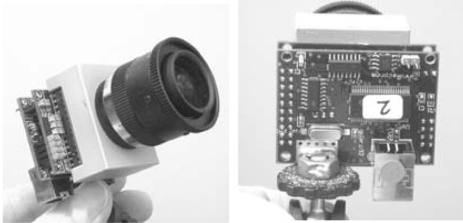
\includegraphics[scale=1.5]{dvsSensor.png} 
		\caption{}
	\end{subfigure}\\
	\begin{subfigure}[t]{0.15\textwidth}
		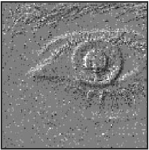
\includegraphics[scale=1.5]{dvsEyeFrame.png}
		\caption{}
	\end{subfigure}
	\begin{subfigure}[t]{0.15\textwidth}
		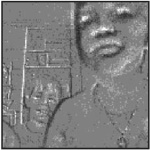
\includegraphics[scale=1.5]{dvsPersonFrame.png}
		\caption{}
	\end{subfigure}
	\begin{subfigure}[t]{0.15\textwidth}
		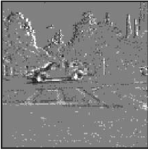
\includegraphics[scale=1.5]{dvsDrivingScene.png}
		\caption{}
	\end{subfigure}
	\caption{(a) - DVS sensor, (b) - Eye shot with DVS sensor, ~7500 events in 300 ms, (c) - Faces, ~8000 events in 26 ms, (d) - Driving scene, ~4000 events in 29 ms as presented by Lichtsteiner et al in \cite{5}}
	\label{dvsSensorFrames}
\end{figure*}

\begin{table}[]
	\centering
	\caption{Specifications of a Dynamic Vision Sensor by Lichtsteiner et al. \cite{5}}
	\begin{tabular}{lllll}
		\cline{1-2}
		 Dynamic range:&  120dB&  \\ 
		 Contrast threshold mismatch:&  2.1\%&  \\
		 Pixel array size:&  128\(\times\)128 pixels of 40\(\mu\)m \(\times\) 40\(\mu\)m&  \\
		 Photoreceptor bandwidth:&  \(\geq\)3 kHz&  \\ 
		 Event saturation rate:&    1 million events per second& \\ 
		 Power consumption:& 23mW& \\ 
		 Minimum latency:& 15\(\mu\)s&\\ \cline{1-2}
	\end{tabular}
\label{tableDVSSpecs}
\end{table}

In Fig. \ref{dvsSensorFrames} the DVS hardware and DVS data frames are depicted. Table \ref{tableDVSSpecs} lists devise properties. In this work a V-REP model of DVS128 sensor provided by iniLabs \cite{6} was used. This model does not exactly match the real hardware as proposed in \cite{5} since simulating DVS with aforementioned specifications is difficult. Instead, the sensor is simulated by comparing subsequent frames of a video stream, and then retaining only pixels, where the absolute difference is greater then a threshold value as done in \cite{7}. However, this method compounded with simulating in time steps undermines the key features of event independence and microsecond temporal resolution of a real DVS sensor. The pixel events are now emitted every simulation time step with the same time stamp and as such the simulated DVS data differs from real data rather significantly as shown by Kaiser et al. \cite{7} in \ref{fig:dvsDiff}. They proceed to argue, that a robust SNN would be able to cope with such inputs. 

\begin{figure}[b]
	\centering
	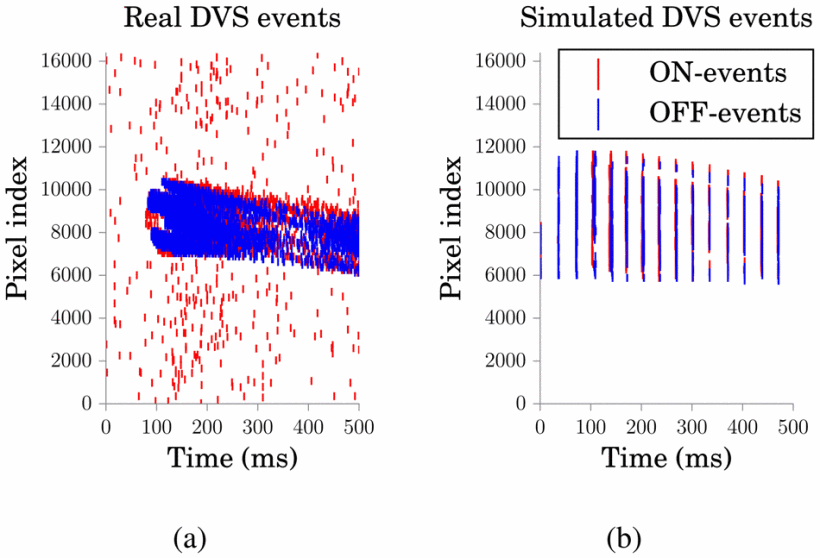
\includegraphics[scale=1]{dvsDifferencesRealVsSim.png}
	\caption{(a) - real DVS data, (b) - simulated DVS data \cite{7}\label{fig:dvsDiff}}
\end{figure}

The DVS model uses AER Protocol to transmit its data. AER Protocol specifies a simple format for event messages: (\(x\), \(y\))-address, ON/OFF state, and a time stamp. The model provided by iniLabs uses 14 bits for address, 1 bit for state, 16 bits for time stamp and leaves 1 bit unused. In this work, in order to simplify simulation, only address information was used. Also, only the walls were made detectable, while the floor and other objects were made invisible for the DVS sensor. The typical simulation DVS frame is shown in Fig. \ref{fig:dvsSimFrame}.

\begin{figure}[h]
	\centering
	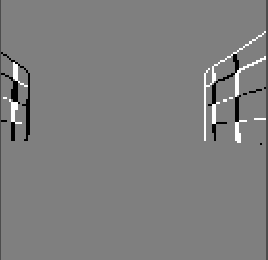
\includegraphics[scale=0.8]{dvsSimFrame.png}
	\caption{Simulated DVS frame\label{fig:dvsSimFrame}}
\end{figure}


\subsection{HiBot ACM-R5 Snake Robot}
ACM-R5 is an amphibious snake-like robot developed by HiBot Corporation \cite{3}. For this robot, a V-REP model is available with default V-REP installation (Fig. \ref{fig:acm-r5}). It is composed of 9 segments connected with 2 revolving joints, that turn round y and z axis, allowing robot to operate in water. 
In this work, the snake robot is only used on a horizontal plane. The joints turn angles are controlled by a child script associated with ACM-R5 in V-REP. In a work by Bing et al.\cite{4} a slithering gate movement model was developed which is used here. The following 2D extended gait equations 

\begin{gather*} 
\alpha(n,\ t)= C+P\cdot A\cdot\sin(\Omega\cdot n+ \omega\cdot t) \label{gateeq}\\ 
P=(\frac{n}{N}\cdot z+y)\in[0,\ 1],\quad \forall n\in[0,\ N]\tag{1},
\end{gather*}

where \(\alpha(n, t)\) is the joint angle of the \(nth\) joint at time \(t\), \(C\) - body shape offset, \(A\) - wave amplitude, \(P\) - linear reduction coefficient,  \(\Omega\) - spatial frequency,  \(\omega\) - time frequency, \(N\) - robot module amount, \(n\) - module subscript, \(y,z\) - linear coefficients govern the motion of the snake-like robot. Slithering gate induces the head module to move with substantial amplitude from side to side while staying directed forward. This can distort DVS image and make learning unstable. In order to minimize that effect, linear reduction coefficient \(P\) modifies wave amplitude \(A\) such that it is minimal at the head module and linearly increases up to the tail module. According to Bing et al. \cite{4} linear reduction modifies shape of the robot from cylinder to frustum and reduces the head swing motion by \(70\%\). The body shape offset \(C\) is a control parameter, added as a bias to \ref{gateeq} control snake turn radius. It is defined as
\begin{gather*}
C = \frac{l_0 \cdot \Sigma_{k=1}^N cos(A\cdot \Sigma_{p=1}^k sin(\Omega \cdot p))}{r}
\end{gather*}

where \(l_0\) is length of a single snake module and \(r\) is the turn radius.

\begin{figure}[h]
	\begin{center}
		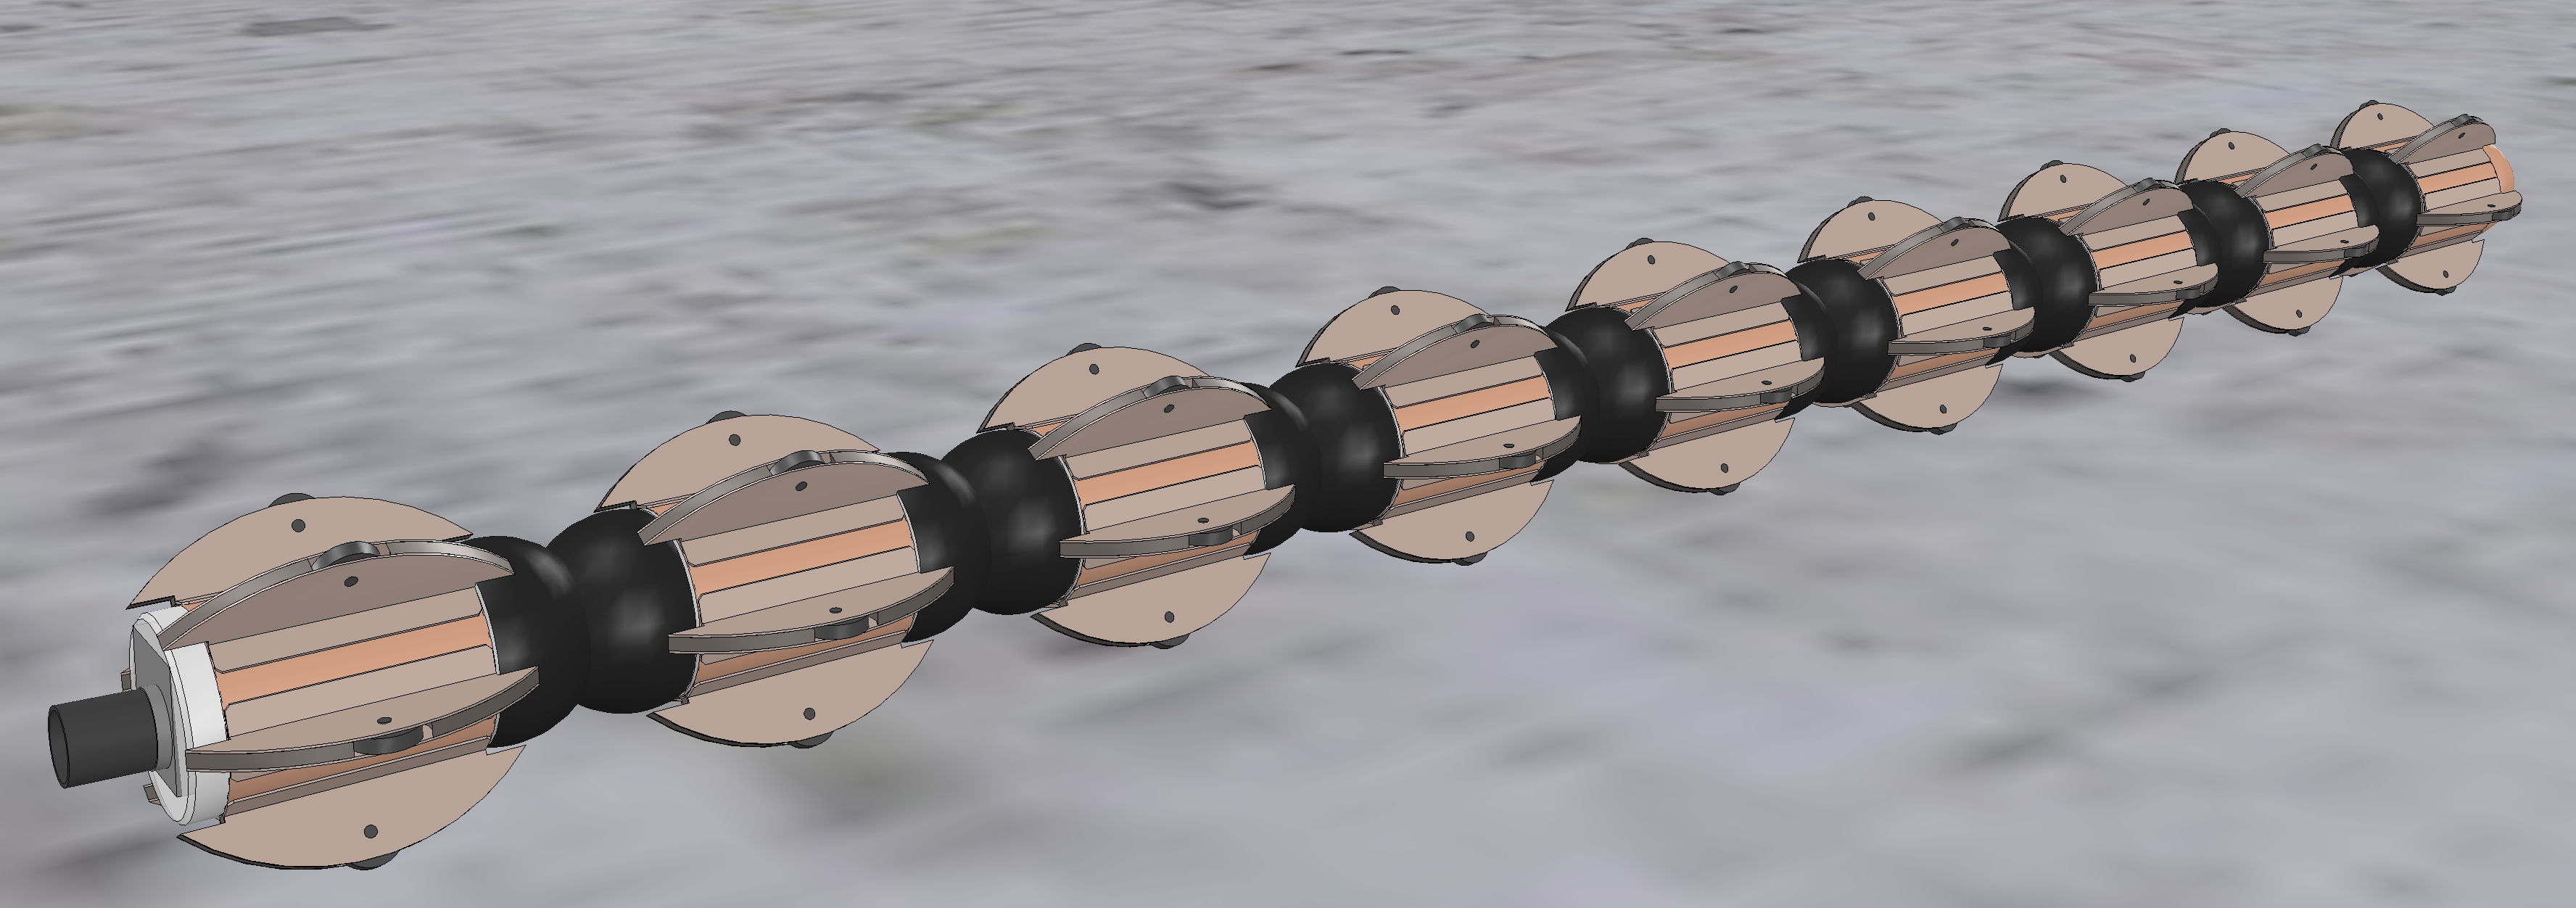
\includegraphics[scale=0.1]{acm-r5.png}
		\caption{ACM-R5 model in V-REP with a DVS\label{fig:acm-r5}}  
	\end{center}
\end{figure}

\section{Simulation Scenarios}\label{simscen}
In order to generate SNN training data and to subsequently test the trained networks two V-REP scenarios were developed. The ACM-R5 model was modified to include a DVS128 sensor as well as 5 proximity sensors mounted on the first (head) module. 
\subsection{Modified ACM-R5 Model}

ACM-R5 model was extended to include DVS sensor and 5 ray-type proximity sensors in its head module. The DVS sensor was used to generate spiking neural network input while the proximity sensors were used to compute reward signal (as explained in Section \ref{rewardSig}). On Fig. \ref{fig:dvsProxyConfig} the configuration of proximity sensors with relation rectangle, bootstrapped by DVS near and far clipping plane as well as perspective angle \(\alpha\) is shown. Proximity sensors are arrayed in such a way, that the angle between left and right sensors match the perspective angle \(\alpha\). The angles between sensors \(\beta\) are all equal. 
\begin{figure}[h]
	\begin{center}
		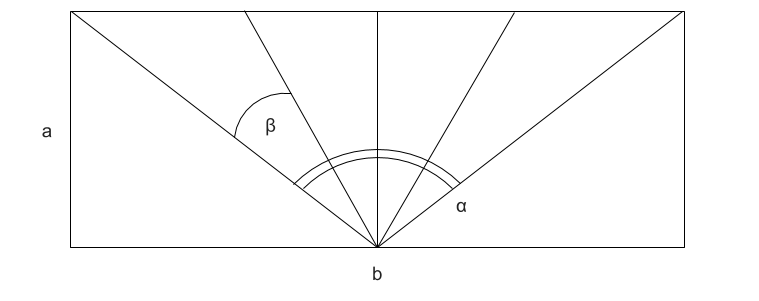
\includegraphics[scale=1]{dvsAndProxyConfig.png}
		\caption{A DVS sensor volume with proximity sensors cutting it into 4 sectors\label{fig:dvsProxyConfig}}  
	\end{center}
\end{figure}

In the Table \ref{tableDVSProxySpecs} the measurements are listed.

\begin{table}[h]
	\centering
	\caption{Proximity sensor position properties}
	\begin{tabular}{lllll}
		\cline{1-2}
		 Outter left proximity sensor detection length:&  \(1.5 m\)&  \\ 
		 Outter right proximity sensor detection length:&  \(1.5 m\)&  \\
		 Inner left proximity sensor detection length:&  \(1.1 m\)&  \\
		 Inner right proximity sensor detection length:&  \(1.1 m\)&  \\ 
		 Perspective angle \(\alpha\):&    100\degree& \\ 
		 Angle between proximity sensors \(\beta\):& 25\degree& \\ 
		 Near to far clipping plane distance \(a\):& \(1 m\)&\\ 
		 Frame length \(b\):& \(1 m\)&\\ \cline{1-2}
	\end{tabular}
\label{tableDVSProxySpecs}
\end{table}

\subsection{Training Scenario}

First V-REP scenario is for SNN training. It consists of 3 different stages with stage 1 and 3 split into 2 phases. Table \ref{tableTrainingScenario1} provides measurements:

\begin{table}[h]
	\centering
	\caption{Training scenario 1 wall measurements}
	\begin{tabular}{lllll}
		\cline{1-2}
		 Wall-to-wall distance:&  \(1.5 m\)&  \\ 
		 Turning radius for outer walls:&  \(10 m\)&  \\
		 Turning radius for inner walls:&  \(5 m\)&  \\
		 Walls height:& \(0.5 m\)&\\
		\cline{1-2}
	\end{tabular}
\label{tableTrainingScenario1}
\end{table}


Robot starts in stage 1, which is realised in 2 phases. In phase 1 it is positioned on the left-hand side of the U-Turn and learns the right U-Turn. Once completed in phase 2 it is set on the right-hand start of the U-Turn to learn the left U-Turn. After successfully completing U-Turn in both directions, it is set on a straight lane (stage 2). Finally, it is moved to complete left turn and subsequently right turn in the stage 3 phase 1 and phase 2 respectively.  The training routine is specified in ACMR child script and makes use of V-REP distance calculation module. Each stage uses dummy objects to calculate the minimal distance between the ACM-R5 robot and itself. If the distance becomes smaller then 2 meters, the current phase is completed and robot is moved to the next phase or stage. In Fig. \ref{fig:vrepScenario1} the starting points of each stage and phase are labelled. Once all stages are completed, the training is stopped by publishing completion message to '/simStopped' topic.

\begin{figure}[h]
	\begin{center}
		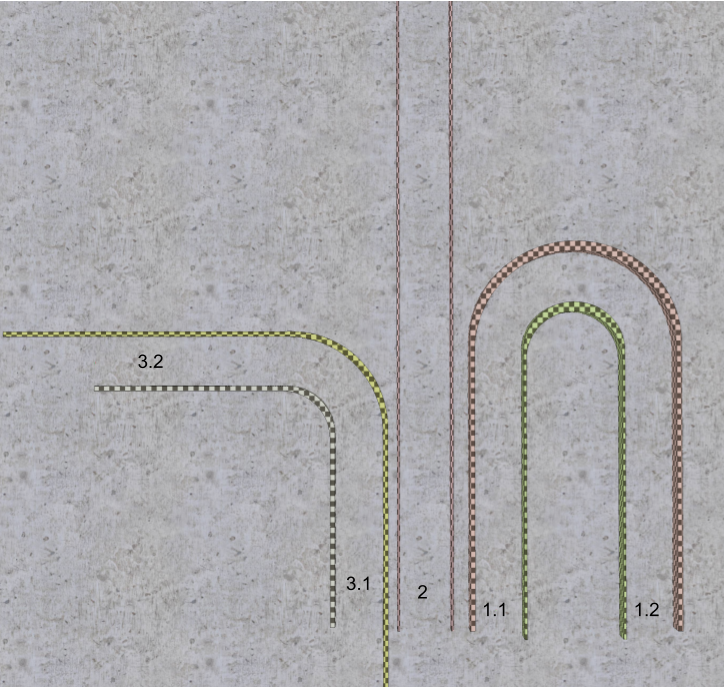
\includegraphics[scale=1]{vrepScenario1.png}
		\caption{V-REP Scenario 1 with stage starting points labelled \label{fig:vrepScenario1}}  
	\end{center}
\end{figure}

\subsection{Testing Scenario}
The testing scenario is used to verify the networks trained in the training scenario. It is similar in form to scenario 1 proposed by Bing et al. \cite{8}. In order to test the ability of trained networks to adapt to a changed world, wall to wall distances, wall heights and textures are modified. In Fig. \ref{fig:vrepScenario2} the different wall-to-wall distance segments are enumerated. The snake robot starts in the segment 1 and moves through subsequent turns.  

\begin{figure}[h]
	\begin{center}
		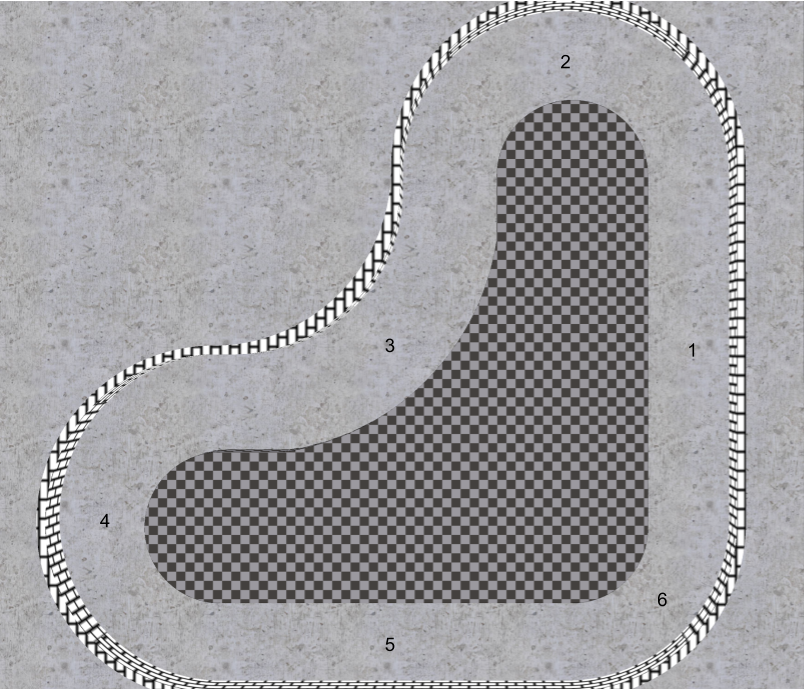
\includegraphics[scale=1]{vrepScenario2.png}
		\caption{V-REP Scenario 2 \label{fig:vrepScenario2}}  
	\end{center}
\end{figure}

Test run is completed, once the robot reaches starting position. For that same approach as in the training scenario is used - once the segment 6 is passed and head module of ACM-R5 is closer to the dummy object then 0.3 meters, simulation completion state is published to '/simStopped' topic. Table \ref{tableTestingScenario2} provides per-segment wall-to-wall distances and wall heights. Additionally, outer wall's texture was changed to a brick wall. 

\begin{table}[h]
	\centering
	\caption{Training scenario 2 wall-to-wall distances for segments 1-6 and wall heights}
	\begin{tabular}{lllll}
		\cline{1-2}
		 Inner wall height:& \(0.35 m\)&\\
		 Outer wall height:& \(0.55 m\)&\\
		 Segment 1:&  \(1.4 m\)&  \\ 
		 Segment 2:&  \(1.7 m\)&  \\
		 Segment 3:&  \(1.8 m\)&  \\
		 Segment 4:& \(1.6 m\)&\\
 		 Segment 5,6:& \(1.4 m\)&\\
		\cline{1-2}
	\end{tabular}
\label{tableTestingScenario2}
\end{table}

\section{Neural Network}\label{nest}
\subsection{NEST Simulator}
The spiking neural networks for this work were developed using NEST Simulator developed by Nest Initiative. NEST provides full-fledged framework for spiking neural network creation and simulation. In this work NEST 2.16 was used to define spiking neural network and simulate it.
\subsection{Transforming DVS output into SNN input}\label{sectionDVStoSNN}

DVS sensor model has resolution of 128\(\times\)128 pixels. As shown in Section \ref{dvsSection} due to simulation environment and model constraints, the pixels are not temporally independent and the data is transmitted every 50ms with the same time stamp. In order to effectively use it as input for the spiking neural network, the events must be spread in time. Bing et al. in \cite{8} proposed a method of adapting the raw DVS output. For the purposes of this work this method was slightly modified. The DVS data is scaled down from 128\(\times\)128 pixles to an 8\(\times\) frame, where each pixel is fused from original pixels with changed state, regardless of polarity. Subsequently the value of each pixel in the new 8\(\times\)8 frame is spread in time by clamping it to maximum value of 300 and using it to set the rate of poisson spike generator connected in one-to-one fashion to parrot neurons with static, unchanging synapses. The steps are shown in Fig. \ref{fig:dvsTransform}

\begin{figure*}[t!]
	\captionsetup{justification=centering}
	\centering
	\begin{subfigure}[t]{0.5\textwidth}
		\centering
		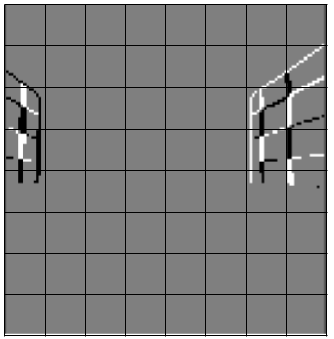
\includegraphics[scale=2]{DvsSimFrameGrid.png} 
		\caption{}
	\end{subfigure}
	\begin{subfigure}[t]{0.3\textwidth}
		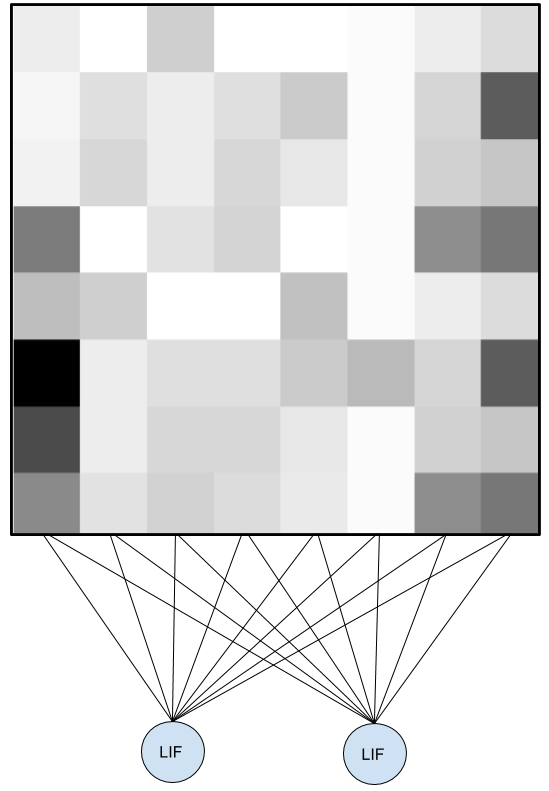
\includegraphics[scale=0.85]{networkConfig.png}
		\caption{}
	\end{subfigure}
	\caption{Scaling of original DVS frame to 8\(\times\)8 frame \\(a) - original simulated frame, (b) - fused 8\(\times\)8 frame \label{fig:dvsTransform}}  
\end{figure*}



\subsection{Spiking Neural Network Architecture}
Following spiking neural network architecture based on Kaiser et al. \cite{7} and Bing et al. \cite{8} was trained using 2 different reward signal functions and reward-modulated STDP schemes. It consists of 8\(\times\)8 Poisson spike generators generating input spikes as discussed in previous section, connected to 8\(\times\) parrot neurons. The input neurons are subsequently connected in all-to-all fashion with dopamine-modulated STDP synpases to 2 LIF action neurons modelling the "turn left" and "turn right" state. The output spikes of action neurons are used to calculate the turning radius of the snake. Instead of generating the dopaminergic signal by exciting a user-specified pool of neurons and using volume transmitter to deliver it to synapses as proposed by Potjans, Wiebke et al.\cite{10}, the neuromodulator concentration \(n\) was set directly in each simulation time step. This trade-off in biological plausibility allows for significant simulation simplification while still maintaining the underlying dynamics of dopamine modulation. For additive scheme, connections to the left action neuron \(conn_{left}\) received and right action neuron \(conn_{right}\) were updated using Eq. \ref{eq:additiveSTDP}, such that the neuromdulator concentration was set to be opposite for left and right connections. For multiplicative scheme, the Eq. \ref{eq:multiplicativeSTDP} was used. The neurons and synapses parameters can be found in 


\section{Controller}\label{controller}
All the parts discussed in previous sections are driven from a PyDev project consisting of training.py, controller.py, environment.py, networkARMSTDP.py, networkMRMSTDP.py and helper files. Following chapters will detail project architecture, V-REP to python controller communication, training and testing flows.

\subsection{Reward Calculation}\label{rewardSig}
In order to train the network a reward signal based on sensory input must be generated. The aim of this work was not only to compare the performance of different learning rules but also to develop a simulation model, that will not depend on any information, that is not directly sensed by the robot. To this purpose, 2 reward functions are proposed and implemented in environment.py. First function uses cubic function of approximation of lane center defined as follows: the distance sensed by left and right proximity sensor was projected on near clipping plane of DVS, center was approximated and then used as variable for the cubic function:
\begin{gather}\label{eq:centerReward}
	d_{left} = p_{left} \cdot cos(50^\circ)\\
	d_{right} = p_{right} \cdot cos(50^\circ)\\
	r = (\frac{d_{left} - d_{right}}{2} - d_{left})^3
\end{gather}
Second function uses all 5 proximity sensors to calculate reward signal as a cubic function of difference between sum of area of triangles formed by outer left, inner left and forward sensor and outer right, inner right and forward sensor. 

\begin{gather}\label{eq:areaReward}
	a_{left} = \frac{1}{2} \cdot p_{left} \cdot p_{innerleft} \cdot cos(25^\circ) + \frac{1}{2} \cdot p_{innerleft} \cdot p_{forward} \cdot cos(25^\circ)\\
	a_{right} = \frac{1}{2} \cdot p_{right} \cdot p_{innerright} \cdot cos(25^\circ) + \frac{1}{2} \cdot p_{innerright} \cdot p_{forward} \cdot cos(25^\circ)\\
	r = (a_{left} - a_{right})^3
\end{gather}

\begin{figure*}[t!]
	\captionsetup{justification=centering}
	\centering
	\begin{subfigure}[t]{0.5\textwidth}
		\centering
		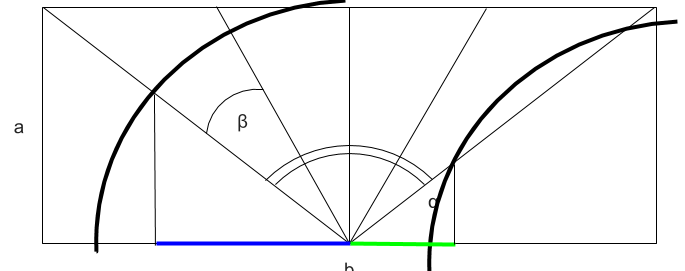
\includegraphics[scale=1]{centerReward.png} 
		\caption{}
	\end{subfigure}
	\begin{subfigure}[t]{0.4\textwidth}
		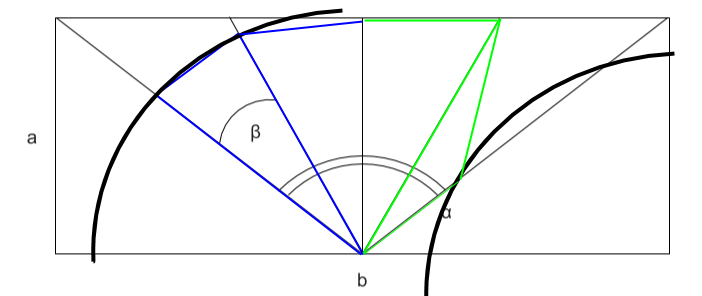
\includegraphics[scale=1]{areaReward.png}
		\caption{}
	\end{subfigure}
	\caption{Reward function \\(a) - center approximation based, (b) - area based \label{fig:reward}}  
\end{figure*}

In Fig. \ref{fig:reward} both functions are depicted. The comparative advantages and drawbacks of both functions are discussed in Chapter \ref{chapter:discussion}.

\subsection{Snake Turning Model}
Snake robot is directly controlled by the difference between \(n_{left}\) and \(n_{right}\) spike count read from left and right action neuron respectively. Justification for that is that robot must learn to turn away from neuroactive regions of the input frame, since a more neuroactive region would induce the respective action neuron to fire more then its counterpart. When travelling between 2 walls it results in a the robot striving to stay in the center but it also induces robot to avoid obstacles.

\subsection{Project Architecture}

The project architecture is same as in RSTDP controller developed by Claus Meschede for his Master's Thesis \cite{11} (Fig. \ref{fig:controllerArch}) and is depicted below. In this work, python 3.7 was used instead of python 2.7 as well as ROS Melodic Morenia and NEST 2.16. The simulation was hosted on an Archlinux machine. Archlinux was chosen due to hardware constraints of the host machine. However, this should not provide any difficulties in replication of this work on a common Ubuntu machine. The workflow of a single controller execution is depicted in Fig. \ref{fig:controlFlow}.

\begin{figure}[h]
	\centering
	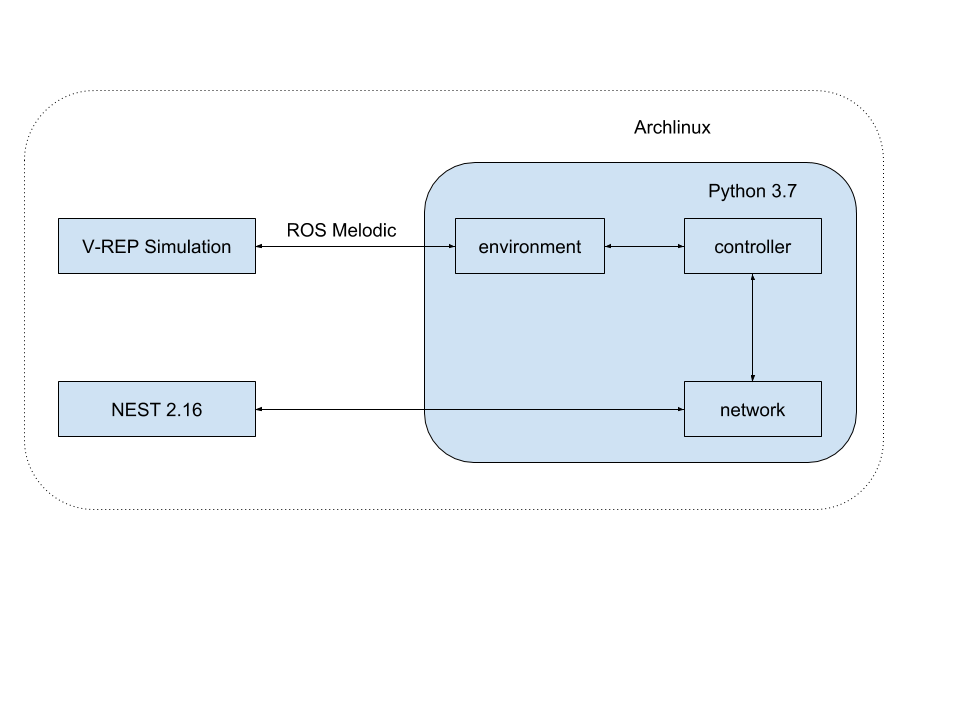
\includegraphics[scale=0.3]{controllerArch.png} 
	\caption{Controller architecture used in this work}
	\label{fig:controllerArch}
\end{figure}
\begin{figure}[h]
	\centering
	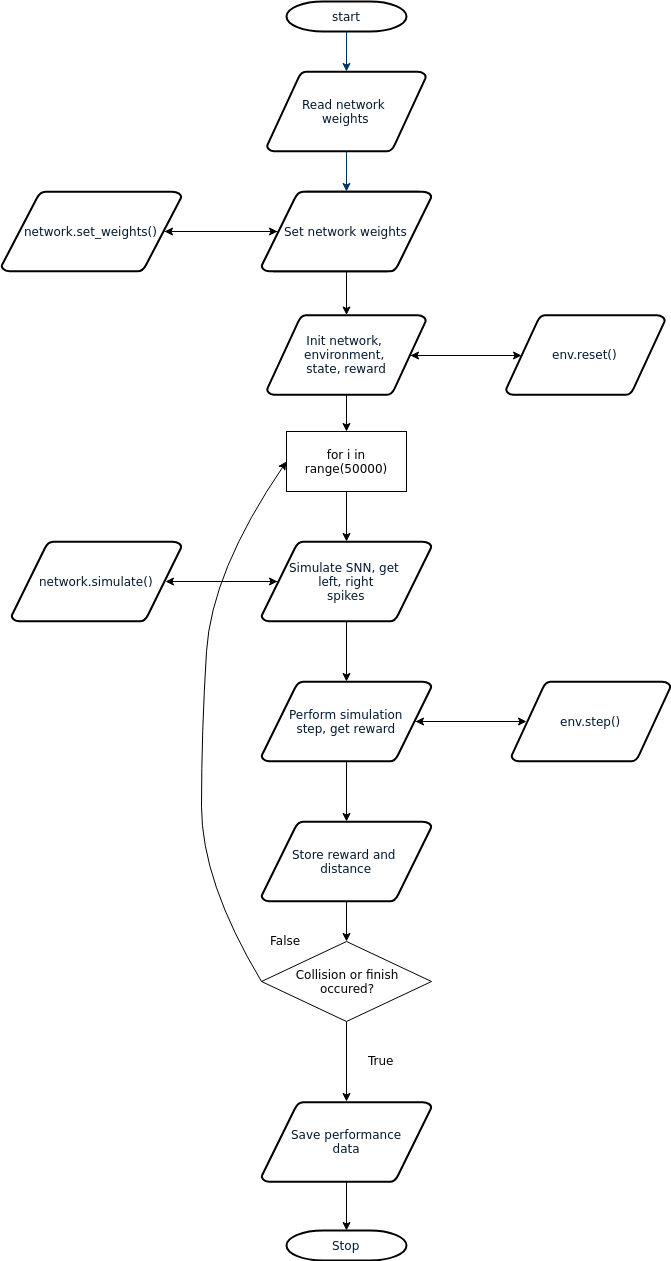
\includegraphics[scale=0.3]{controlFlow.png} 
	\caption{Testing flow}
	\label{fig:controlFlow}
\end{figure}

\subsection{V-REP to Controller communication}
The communication between V-REP simulation and python controller is handled via ROS messages. Both python environment handler and V-REP ACM-R5 child script define a number of ROS publishers and subscribers. On the V-REP side, proximity sensors data, DVS data, collision flag and simulation completion flag are published, while simulation itself subscribes to environment's handler radius and reset topics. Environment handler subscribes to data topics provided by V-REP simulation and handles the incoming data.